\section{Introduction to GPU computing (1)}

\subsection{Short reminder}
The saturation shown by Moore's law limits the possible performance of a single processor (faster clock means higher dissipation, which leads to the so-called power wall). We then find ourselves in need of parallel programming, which is no longer something for supercomputers since all processors nowadays are multicore. Several problems can be split into smaller tasks to be solved concurrently, and in any case the maximum speed-up is not linear, but it depends on the serial part of the code, as described by Amdahl's law. The situation can improve if the amount of parallelizable part depends on the resources, as stated by Gustafson's Law.

\subsection{What are GPUs?}

\textbf{Graphics Processing Units (GPUs)} are processors dedicated to parallel programming for graphical applications. Rendering, image transformation, ray tracing, etc\dots are typical applications where parallelization helps a lot. We will get to a more technical definition later. For now, let's focus on the basic functioning of a GPU. 

Here's the \textbf{standard GPU pipeline} (as shown in the following figure):
\begin{enumerate}
    \item Vertex/Index buffers: The input is "assembled" by the GPU by using fixed vertices (points on the image) and their connections into triangles;
    \item Vertex shading: The position of every vertex is calculated on screen based on the original position and camera viewpoint;
    \item Rasterization: The pixel-by-pixel color values are retrieved;
    \item Pixel shading: The colour is given to every pixel based on texture properties (material, light, etc\dots);
    \item Rendering: The output is written to the render target and then copied into the computer memory.
\end{enumerate}

\begin{center}
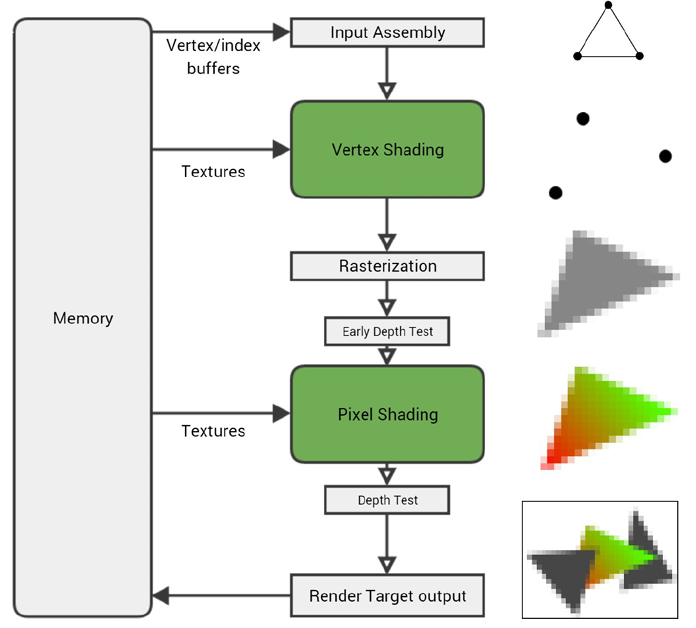
\includegraphics[width=0.5\textwidth]{figuresP/lesson_parallel_3B_pag_6.png}
\end{center}

From this oversimplified scheme you should get two important concepts: each triangle that creates an image is independent of each other (and so different processors can work simultaneously on each triangle) and the exchange of data between the memory and the GPU is constant and needs to be fast. Modern GPUs don't exactly work like this anymore, but the basic idea remains the same.

In other words, the graphics pipeline requires a huge amount of arithmetic on independent data (this includes transforming positions, generating pixel colors, and applying material properties and light situations to every pixel). The hardware requires the ability to access memory simultaneously and contiguously (considering that bandwidth is more important than latency) and needs floating-point and fixed-function logic.

We then get to the canonical definition of a GPU: it is "\textit{a single-chip processor with integrated transform, lightning, triangle setup/clipping and rendering engines that is capable of processing a minimum of 10 million polygons per second}". Apart from the hardware components specified, this definition is based on the capability of the GPU to process the triangles we were previously talking about. In fact, GPUs were invented in 1997 just for image processing ($\equiv$ "to work with triangles") and we had to wait until 2007 before NVIDIA opened the possibility to use them for generic computing (GPGPU). In 2008 a consortium of different firms decided to introduce a common multiplatform language for manycore computing called \textbf{OpenCL}.

We will not be using OpenCL during this course, but CUDA (which is used specifically for NVIDIA GPUs). These two frameworks are very similar (so it will be very easy to switch to OpenCL if you want to), but CUDA is better documented and better for learning the basics.

GPUs are a way to cheat Moore's law thanks to their SIMD/SIMT (\textit{Single Instruction Multiple Threads}, we will see what this means) parallel architecture. They offer very high computing power for vectorizable problems, with an impressive derivative that is almost a factor of 2 in each generation. Thanks to continuous development (due to higher and higher economic interest in video games and such), it is easy to have a desktop PC with teraflops\footnote{As you might already know, the number of FLOPS (\textit{Floating Point Operations per Second}) is a measurement of the computing power of a processor. Theoretically, it is defined as:
$$ \text{FLOPS} = \text{clock frequency} \cdot \text{\# cores} \cdot \text{\# operation per cycle} $$
but of course this formula doesn't take into account several things. The real estimation is made experimentally by using standard packages (LINPACK, LAPACK) and other metrics have been invented to avoid the limitations of FLOPS in measuring the computing power, such as SPECint and SPECfp.} of computing power, with thousands of cores. This leads to several applications in \textit{high-performance computing} (HPC), simulation, scientific computing etc\dots

Take a look at the specifics of some of the GPUs on the market in the tables below, and note for example the great number of cores that each one has. 

\begin{table}[H]
\centering
\resizebox{\textwidth}{!}{
\begin{tabular}{|l|l|l|l|l|l|l|}
\hline
\textbf{Tesla GPU} & \textbf{Fermi GF100} & \textbf{Fermi GF104} & \textbf{Kepler GK104} & \textbf{Kepler GK110} & \textbf{Maxwell GM200} & \textbf{Pascal GP100} \\ \hline
Compute Capability & 2.0 & 2.1 & 3.0 & 3.5 & 5.2 & 6.0 \\ \hline
Streaming Multiprocessors (SMs) & 16 & 16 & 8 & 15 & 24 & 56 \\ \hline
FP32 CUDA Cores/SM & 32 & 48 & 192 & 192 & 128 & 64 \\ \hline
FP32 CUDA Cores & 512 & 384 & 1536 & 2880 & 3072 & 3584 \\ \hline
FP64 Units & 256 & 32 & 64 & 960 & 96 & 1792 \\ \hline
Threads/Warp & 32 & 32 & 32 & 32 & 32 & 32 \\ \hline
Max Warps/Multiprocessor & 48 & 48 & 64 & 64 & 64 & 64 \\ \hline
Max Threads/Multiprocessor & 1536 & 1536 & 2048 & 2048 & 2048 & 2048 \\ \hline
Max Thread Blocks/Multiprocessor & 8 & 8 & 16 & 16 & 32 & 32 \\ \hline
32bit-Registers/Multiprocessor & 32768 & 32768 & 65536 & 65536 & 65536 & 65536 \\ \hline
Max Registers/Thread & 63 & 63 & 63 & 255 & 255 & 255 \\ \hline
Max Threads/Thread Block & 1024 & 1024 & 1024 & 1024 & 1024 & 1024 \\ \hline
Shared Memory Size Configs & 16 KB/48 KB & 16 KB/48 KB & 16 KB/32 KB/48 KB & 16 KB/32 KB/48 KB & 96 KB & 64 KB \\ \hline
Hyper-Q & No & No & No & Yes & Yes & Yes \\ \hline
Dynamic Parallelism & No & No & No & Yes & Yes & Yes \\ \hline
Unified Memory & No & No & No & No & No & Yes \\ \hline
Pre-Emption & No & No & No & No & No & Yes \\ \hline
\end{tabular}
}
\end{table}

\begin{table}[H]
\centering
\resizebox{\textwidth}{!}{%
\begin{tabular}{|l|l|l|l|l|}
\hline
\textbf{GPU} & \textbf{NVIDIA H100 (GH100)} & \textbf{NVIDIA A100 (GA100)} & \textbf{NVIDIA Tesla V100 (GV100)} & \textbf{NVIDIA Tesla P100 (GP100)} \\ \hline
Transistors & 80B & 54.2B & 21.1B & 15.3B \\ \hline
Die Size & 814 mm² & 828 mm² & 815 mm² & 610 mm² \\ \hline
Architecture & Hopper & Ampere & Volta & Pascal \\ \hline
Fabrication Node & TSMC N4 & TSMC N7 & 12nm FFN & 16nm FinFET+ \\ \hline
GPU Clusters & 132/114 & 108 & 80 & 56 \\ \hline
CUDA Cores & 16896/14592 & 6912 & 5120 & 3584 \\ \hline
L2 Cache & 50MB & 40MB & 6MB & 4MB \\ \hline
Tensor Cores & 528/456 & 432 & 320 & N/A \\ \hline
Memory Bus & 5120-bit & 5120-bit & 4096-bit & 4096-bit \\ \hline
Memory Size & 80 GB HBM3/HBM2e & 40/80GB HBM2e & 16/32 GB HBM2 & 16GB HBM2 \\ \hline
TDP & 700W/350W & 250W/300W/400W & 250W/300W/450W & 250W/300W \\ \hline
Interface & SXM5/ PCIe Gen5 & SXM4/PCIe Gen4 & SXM2/PCIe Gen3 & SXM/PCIe Gen3 \\ \hline
\end{tabular}%
}
\end{table}

\subsection{CPU vs GPU: designs and advantages}

Both CPUs and GPUs are components of about 5 cm $\times$ 5 cm, but their designs are very different and tailored for their specific applications. 

Take a look at a standard 4-core CPU in the following figure. It relies on multilevel and large caches to convert long latency memory access to short latency cache access and uses branch prediction to reduce latency in branching. It adopts Instruction level parallelism (ILP) with powerful ALUs and includes complex memory management and a large control part. In other words, a \textbf{CPU should have a latency-oriented design}. That's intuitive as it is not only used for computation, but for many other operations that require a nearly instant response for the user (e.g. if you move the mouse you want the icon on your screen to move as fast as possible). 

\begin{center}
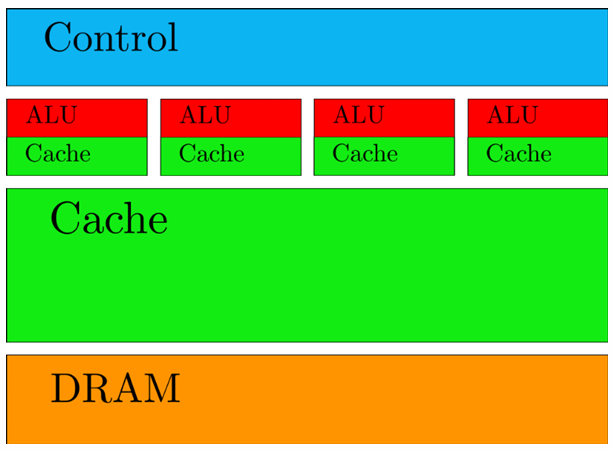
\includegraphics[width=0.3\textwidth]{figuresP/lesson_parallel_3B_pag_15.png}
\end{center}

Instead, a GPU relies on SIMT/SIMD architecture and uses SMX (Streaming Multiprocessors) to execute kernels. It exploits thread-level parallelism with massive threading to hide the latency and features limited caching, primarily to boost memory throughput, and limited control (no branch prediction, but branch predication). That means that every \textbf{GPU has a throughput-oriented design} to maximize its computing capabilities. 

\begin{center}
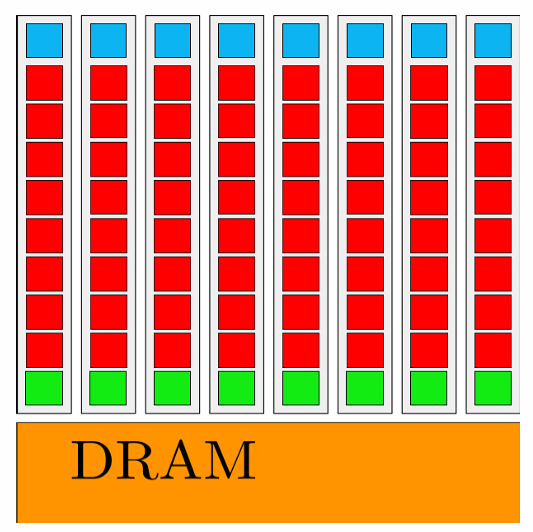
\includegraphics[width=0.3\textwidth]{figuresP/lesson_parallel_3B_pag_16.png}
\end{center}

Below you will find a schematic comparison of the characteristics of a generic CPU and GPU and a table with the specifics of a real CPU and a GPU of the same generation.

\begin{center}
    % Prima colonna: CPU
    \begin{minipage}[t]{0.45\textwidth}
        \centering
        \underline{CPU}\par
        \vspace{0.5em}
        \normalsize
        \begin{itemize}
            \item[+] Large main memory
            \item[+] Fast clock rate
            \item[+] Large caches
            \item[+] Branch prediction
            \item[+] Powerful ALU
            \item[-] Relatively low memory bandwidth
            \item[-] Cache misses costly
            \item[-] Low performance per watt
        \end{itemize}
    \end{minipage}\hfill
    % Seconda colonna: GPU
    \begin{minipage}[t]{0.45\textwidth}
        \centering
        \underline{GPU}\par
        \vspace{0.5em}
        \normalsize
        \begin{itemize}
            \item[+] High bandwidth main memory
            \item[+] Latency tolerant (parallelism)
            \item[+] More compute resources
            \item[+] High performance per watt
            \item[-] Limited memory capacity
            \item[-] Low per-thread performance
            \item[-] Extension card
        \end{itemize}
    \end{minipage}
\end{center}

\begin{center}
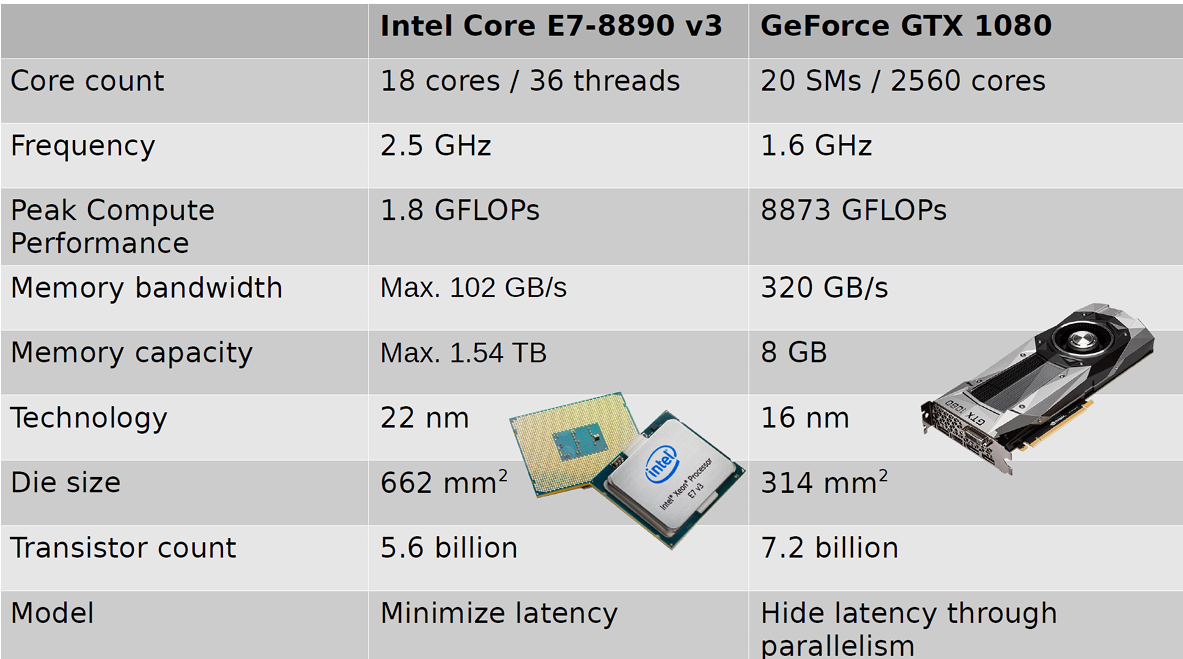
\includegraphics[width=0.6\textwidth]{figuresP/lesson_parallel_3B_pag_19.png}
\end{center}

The winning application uses both CPUs and GPUs, as suggested by Amdahl's law: CPUs are used for sequential parts (they can be 10$\times$ faster than GPUs for sequential code), while GPUs are used for parallel ones, where throughput is fundamental (they can be 100$\times$ faster than CPUs for parallel code). As we will see, what causes the most latency is the exchange of data between these components, and we will learn how to reduce it as much as possible. 

\subsection{Single Instruction Multiple Threads (SIMT) architecture}

\begin{center}
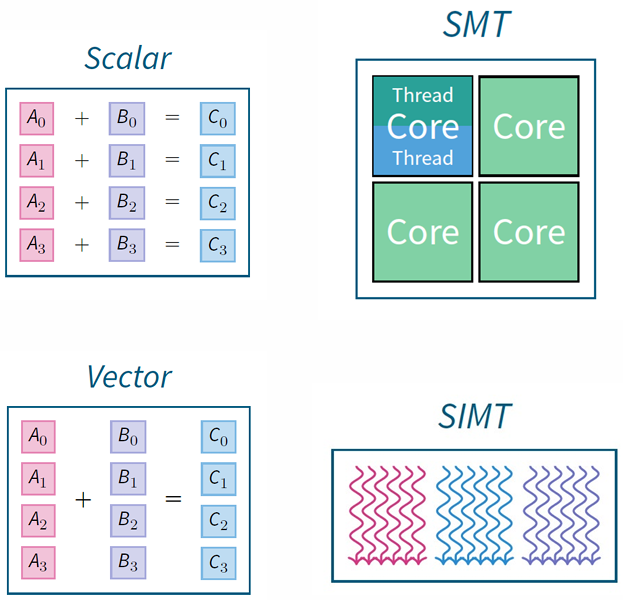
\includegraphics[width=0.35\textwidth]{figuresP/lesson_parallel_3B_pag_21.png}
\end{center}

A SIMD architecture is not the right choice for a GPU. In a SIMD multicore processor, we have to execute the same instruction ($\equiv$ the same line of code, the same thread) on different pieces of data for each core, so they cannot work completely independently. We will see in the next lesson that a GPU is composed of many multiprocessors that actually work as a SIMD architecture, similarly to a multicore CPU. However, each multiprocessor can execute different parts of the same program or completely different programs. That's what we call a \textbf{Single Instruction Multiple Threads (SIMT)} architecture.